% =====================================================================
%  Chapter 6 --- Deployment, API, Dashboard & Azure Operations
% =====================================================================
\chapter{Deployment, API, Dashboard and Azure Operations}
\label{chap:deploy}

\section{Introduction}
The evaluation of Chapter~\ref{chap:model} has confirmed the readiness of the K-Means segmentation and of the Isolation Forest risk score for industrialization. The present chapter executes the deployment phase of CRISP-DM. The chapter describes the deployment strategy, the API and the dashboard exposing the model outputs, the integration with the PostgreSQL warehouse, the cron-driven automation, the monitoring and alerting layer, and finally the Microsoft Azure infrastructure on which the platform runs --- with a particular focus on the secure remote collaboration setup (SSH tunnelling, IP allowlist on the Network Security Group, service accounts).

\section{Deployment strategy}

\subsection{Industrialization principles}
Three principles guide the industrialization. The first one is the \emph{freshness} of the analytical outputs, with a target latency of less than ten minutes between the appearance of an event in the source platform and its visibility in the marts. The second one is the \emph{idempotency} of every step, which allows safe replays. The third one is the \emph{observability}, which guarantees that any incident is detected and diagnosed without manual inspection.

\subsection{Operating modes}
The pipeline supports three operating modes accessible through a single command-line entry point (\texttt{scripts/run\_batch.py}):

\begin{itemize}
    \item \texttt{--mode bootstrap}: one-off DDL and full-refresh of the dimensions and state tables.
    \item \texttt{--mode backfill}: chunked historical replay of the staging tables (default chunk: 30 days).
    \item \texttt{--mode incremental}: default operating mode, processing the slice strictly after the watermark, scheduled every five minutes.
\end{itemize}

\section{Microsoft Azure infrastructure}

\subsection{Azure Virtual Machine}
The platform is hosted on a Microsoft Azure Linux virtual machine. The VM hosts, on the same operating system, the analytical PostgreSQL instance, the Python virtual environment, the Prefect flow, the API process, the BI dashboard process, the cron entry and the system journal. The git repository of the project is cloned into \texttt{/opt/accent-fleet-analytics} and a dedicated Linux user (\texttt{azureuser}) owns the runtime artefacts.

\subsection{Network Security Group and IP allowlist}
The VM is associated with an Azure Network Security Group that closes every public port except SSH (port 22), and the SSH port is itself restricted to an explicit allowlist of source IP addresses corresponding to the development workstations of the team and to the office network of \hostorg. This combination ensures that no PostgreSQL port, no API port and no dashboard port is exposed to the public internet.

\subsection{Secure remote collaboration via SSH tunnelling}
Day-to-day collaboration of the team relies on SSH tunnelling. Each team member opens a local tunnel that forwards the local PostgreSQL port to the remote port on the VM, as illustrated in Listing~\ref{lst:ssh-tunnel}. The notebooks and the local clients then connect to \texttt{localhost:5432} as if the database were running locally, while the actual traffic is encrypted by SSH.

\begin{lstlisting}[style=bash,caption={Opening an SSH tunnel from a developer workstation to the Azure VM.},label={lst:ssh-tunnel}]
# Forward local 5432 -> remote 5432 over SSH
ssh -i ~/.ssh/azure_id_ed25519 \
    -L 5432:localhost:5432 \
    -N \
    azureuser@<vm-public-ip>
\end{lstlisting}

\subsection{Service accounts}
Three categories of accounts coexist on the VM: \emph{personal accounts} for human users (e.g.~\texttt{alice}, \texttt{bob}), used only through SSH key authentication; an \emph{automation account} (\texttt{azureuser}) used by cron and by the systemd services; and a \emph{database service account} (\texttt{accent\_pipeline}) used by the pipeline to authenticate against PostgreSQL, with credentials externalized in an environment file.

\section{PostgreSQL integration}

\subsection{Local PostgreSQL on the VM}
The analytical PostgreSQL is provisioned in version~16 on the VM, with the three schemas \texttt{staging}, \texttt{warehouse} and \texttt{marts}, plus the operational tables \texttt{etl\_watermark}, \texttt{etl\_run\_log} and \texttt{quarantine\_rejected}. The instance listens only on \texttt{localhost}, which is why remote access is mediated by the SSH tunnel described above.

\subsection{Connection management}
The pipeline manages the database connection through a \texttt{SQLAlchemy} engine with a connection pool, an automatic ping before each transaction (\texttt{pool\_pre\_ping}) and an explicit timeout. The credentials are read from a \texttt{.env} file owned by \texttt{azureuser}, with restrictive file permissions.

\subsection{Backups and snapshots}
A nightly logical backup of the analytical database is exported through \texttt{pg\_dump} and rotated through a seven-day retention. A weekly full snapshot of the disk is configured at the Azure infrastructure level and is retained for four weeks.

\section{API and backend}

\subsection{API design}
The API is implemented with FastAPI~\cite{fastapi2024} and exposes a small number of endpoints, summarized in Table~\ref{tab:api-endpoints}. Authentication is handled through API keys associated with the consumer applications.

\begin{table}[h]
\centering
\caption{API endpoints exposed by the platform.}
\label{tab:api-endpoints}
\begin{tabular}{|l|l|p{6.5cm}|}
\hline
\textbf{Method} & \textbf{Endpoint} & \textbf{Description} \\
\hline
GET & \texttt{/health}                            & Liveness probe. \\
GET & \texttt{/devices/\{id\}/risk}               & Latest risk score and band of a device. \\
GET & \texttt{/devices/\{id\}/cluster}            & Latest cluster assignment of a device. \\
GET & \texttt{/tenants/\{id\}/leaderboard}        & Top-N high-risk devices of a tenant. \\
GET & \texttt{/tenants/\{id\}/kpi}                & Tenant-month KPI bundle. \\
POST& \texttt{/admin/refresh}                     & Force an off-cycle incremental run. \\
\hline
\end{tabular}
\end{table}

\subsection{Backend architecture}
The API is served by Uvicorn behind an Nginx reverse proxy bound to \texttt{127.0.0.1}. A systemd unit ensures the API restarts automatically after a crash or after a VM reboot. The API queries the marts and views directly through \texttt{psycopg2}, with prepared statements and a small connection pool.

\subsection{Reverse proxy and TLS}
The Nginx reverse proxy listens on port 443 and terminates TLS with a certificate provisioned through Let's Encrypt. It forwards the HTTPS traffic to the local Uvicorn process. Access logs are written to the system journal under a dedicated tag.

\section{Dashboard and frontend}

\subsection{Dashboard implementation}
The dashboard is implemented with Streamlit (or, equivalently, Plotly Dash) and is served as a systemd unit, behind the same Nginx reverse proxy as the API. The dashboard queries the BI views (\texttt{v\_executive\_dashboard}, \texttt{v\_operational\_dashboard}, \texttt{v\_maintenance\_dashboard}, \texttt{v\_fleet\_risk\_dashboard}) through a read-only database connection.

\subsection{Pages and visualizations}
The dashboard is organized in five pages: the executive overview (tenant-month KPIs and rolling deltas), the operational view (daily KPIs and seven-day rolling), the maintenance leaderboard, the risk heatmap (cluster $\times$ band $\times$ tenant) and the device-detail page (history of the risk score, cluster trajectory, alerts). Figure~\ref{fig:dashboard} sketches the architecture of the dashboard.

\begin{figure}[h]
\centering
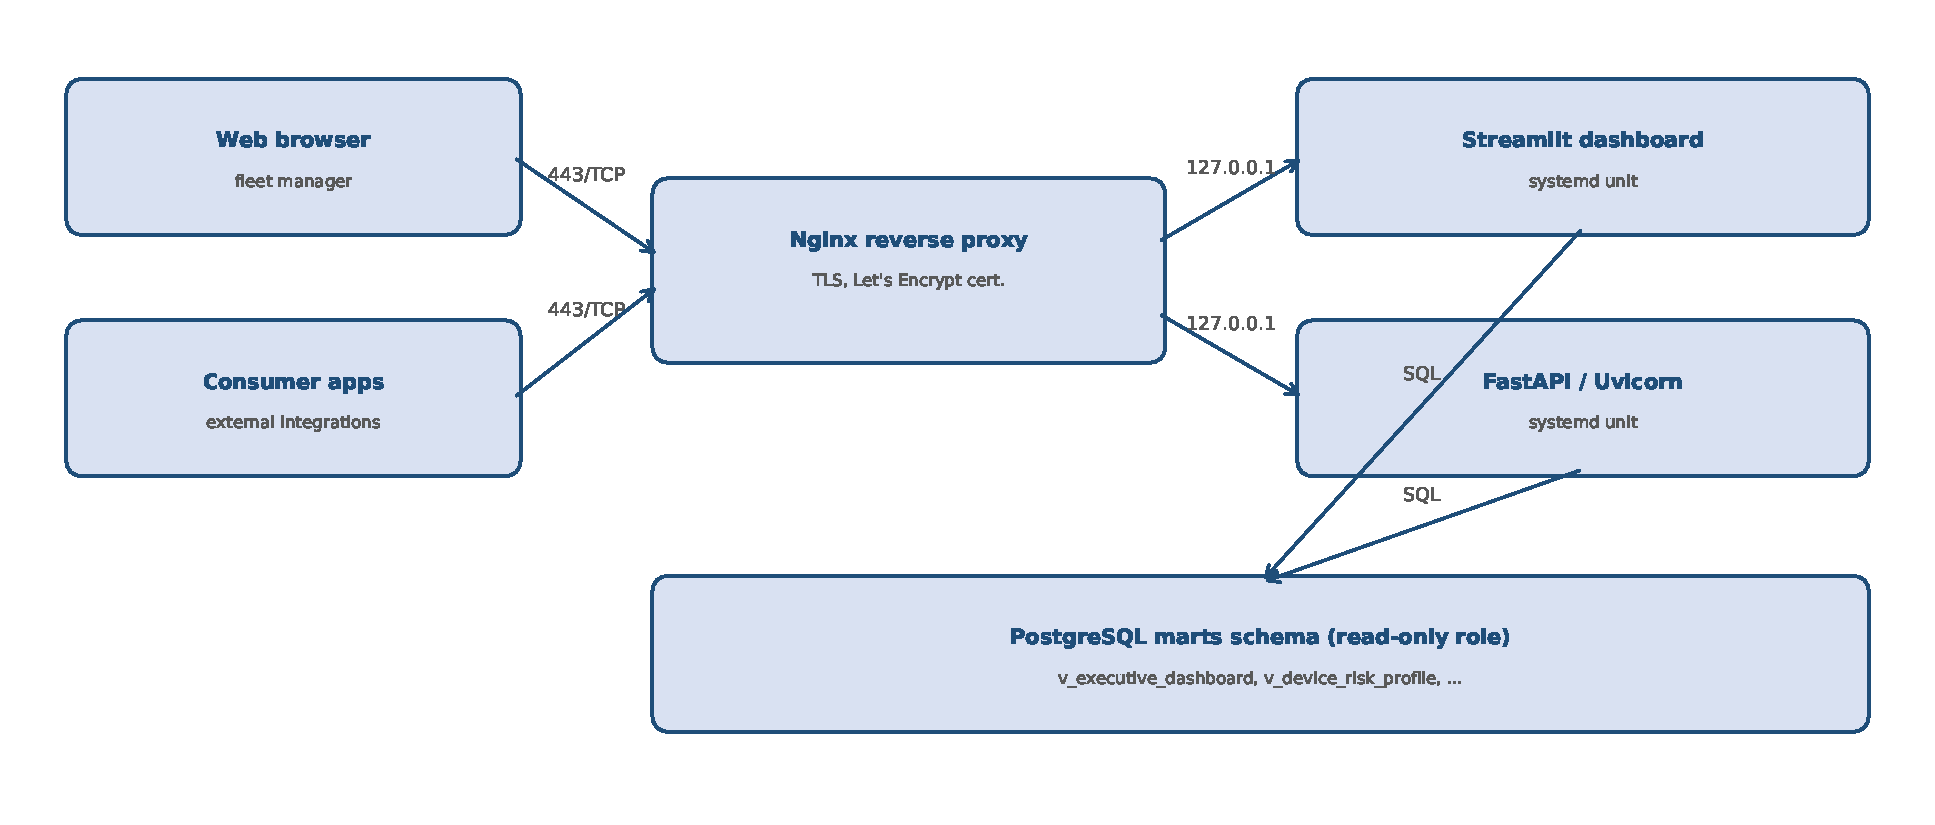
\includegraphics[width=0.85\textwidth]{figures/dashboard_architecture.pdf}
\caption{Architecture of the BI dashboard.}
\label{fig:dashboard}
\end{figure}

\section{Automation}

\subsection{Cron entry}
The incremental mode is triggered every five minutes by a cron entry installed under \texttt{/etc/cron.d/accent-fleet}. The entry calls the pipeline through the Python virtual environment of the project and pipes the standard output and the standard error to the system journal under the tag \texttt{accent-fleet}, as shown in Listing~\ref{lst:cron}.

\begin{lstlisting}[style=bash,caption={Cron entry triggering the incremental pipeline every five minutes.},label={lst:cron}]
*/5 * * * * azureuser cd /opt/accent-fleet-analytics && \
    /opt/accent-fleet-analytics/.venv/bin/python scripts/run_batch.py \
    --mode incremental 2>&1 | logger -t accent-fleet
\end{lstlisting}

\subsection{Prefect flow}
Internally, the pipeline is implemented as a Prefect flow defined in \texttt{src/accent\_fleet/pipeline/flow.py}. The flow chains the extraction tasks, the cleaning rule engine, the loading of dimensions and facts, the materialization of the marts, the validation suite and the export of the model artefacts. Each task is idempotent and emits structured logs.

\subsection{Backfill orchestration}
The backfill mode reuses the same Prefect flow but iterates over fixed-size chunks (default of 30~days) of the staging history. The mode is invoked manually by an operator after a schema change, after a model retraining or after a substantial cleaning-rule revision.

\section{Monitoring and alerting}

\subsection{Run log and lineage}
Every pipeline execution writes a row in \texttt{warehouse.etl\_run\_log}, with the run identifier, the operating mode, the start and end timestamps, the status and the per-fact processed row counts. This table is the principal observability surface of the platform.

\subsection{Data quality monitoring}
The validation suite (\texttt{V1}--\texttt{V8}) is executed at the end of every cycle, and its quantitative outcomes are persisted in a dedicated table. A time series of the data quality measurements is plotted in the executive dashboard.

\subsection{Model drift monitoring}
Model drift is monitored by tracking, on a rolling basis, the proportions of device-months in each K-Means cluster and in each risk band. A statistically significant deviation triggers an alert and motivates a retraining.

\subsection{Alerting}
The alerting layer is implemented in \texttt{src/accent\_fleet/monitoring/} and watches three signals: pipeline failures (status of the run log), data-quality regressions (validation suite) and model drift. When a threshold is crossed, a notification is sent to the operations channel (Slack webhook or e-mail).

\subsection{Operations runbook}
A short runbook documents the manual procedures: how to inspect the run log, how to trigger a backfill, how to restart the API or the dashboard, how to rotate the database credentials and how to renew the TLS certificate. The runbook is reproduced in Appendix~\ref{app:azure}.

\section{Production deployment workflow}

\subsection{Code deployment}
The deployment of new code follows a simple workflow: a pull request is reviewed and merged on the \texttt{main} branch of the git repository; the operator pulls the new commits into \texttt{/opt/accent-fleet-analytics} on the VM; the dependencies are upgraded if needed; the API and the dashboard systemd units are restarted; and the next cron cycle exercises the new pipeline.

\subsection{Database migrations}
DDL changes follow a versioned migration pattern. Every change is shipped as a numbered SQL file under \texttt{sql/} and is applied by the bootstrap mode of the pipeline (or by a manual \texttt{psql} invocation under operator control). The migration scripts are idempotent: a re-execution does not corrupt the schema.

\subsection{Model deployment}
Model deployment relies on the artefact store described in Chapter~\ref{chap:model}. A new model is published as a versioned \texttt{joblib} artefact in a dedicated directory of the VM. The API picks up the most recent artefact at startup or upon receipt of an explicit reload signal.

\subsection{Diagram of the deployment pipeline}
The deployment pipeline is summarized in Figure~\ref{fig:deploy-pipeline}.

\begin{figure}[h]
\centering
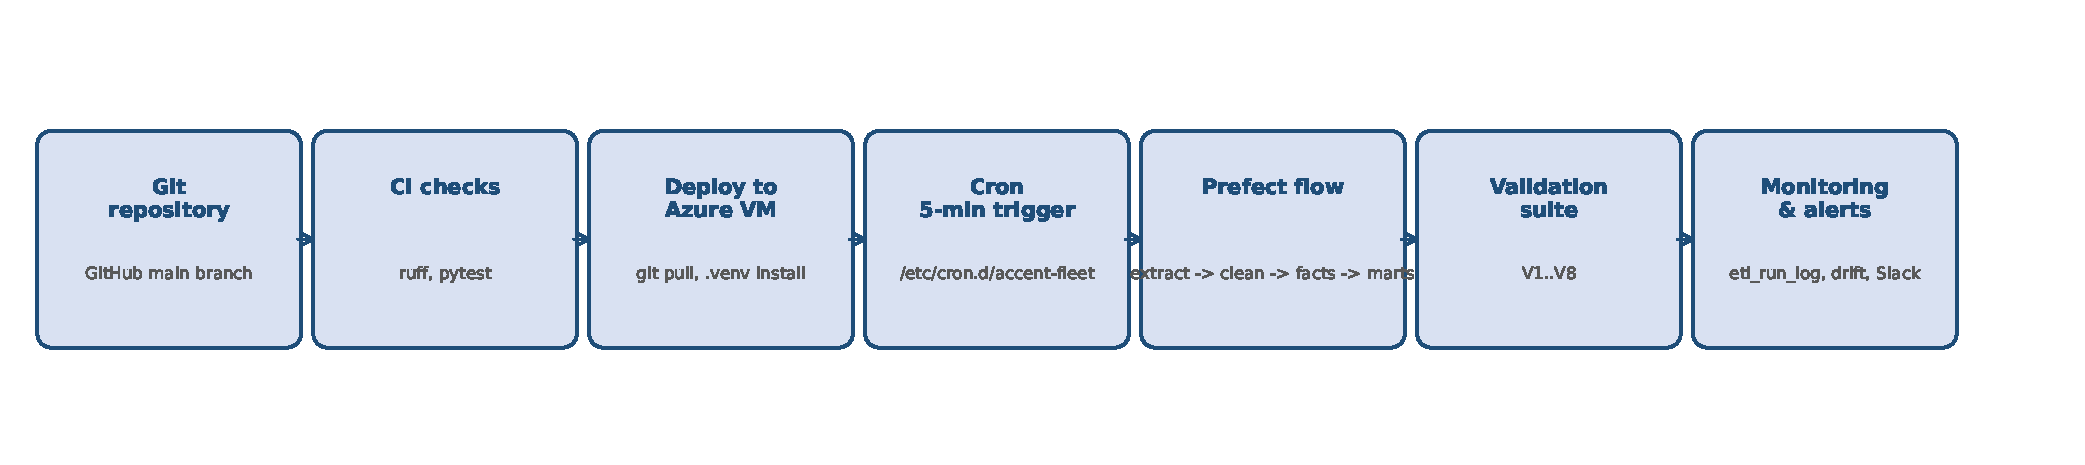
\includegraphics[width=0.95\textwidth]{figures/deployment_pipeline.pdf}
\caption{End-to-end deployment pipeline of the platform.}
\label{fig:deploy-pipeline}
\end{figure}

\section{Conclusion}
This chapter has formalized the deployment of the data engineering and machine learning platform on the Microsoft Azure infrastructure, with explicit attention to the secure remote collaboration setup (SSH tunnelling, IP allowlist on the Network Security Group, service accounts), the API and the BI dashboard, the cron-driven automation, and the layered monitoring and alerting plan. The end-to-end CRISP-DM cycle is therefore brought to its operational completion. The general conclusion that follows synthesizes the deliverables, the lessons learned and the perspectives opened by the project.
